	% Tableau Charcot
\begin{frame}{Domaine impactant dans les écrits de Charcot : \textbf{hystérie}}
	\vspace*{-3mm}
	\begin{table}[h]
		\resizebox{\textwidth}{!}{%
			\centering
			\begin{tabular}{|l|r|r|r|r|r|}
				\hline
				\multicolumn{1}{|c|}{\textbf{Terme}}
				&	\multicolumn{1}{c|}{\textbf{TF-IDF} (\textit{TermSuite})} & 	\multicolumn{1}{c|}{\textbf{TF-IDF}} & 	\multicolumn{1}{c|}{\textbf{BM25}} & 	\multicolumn{1}{c|}{\textit{\textbf{PatternRank}}} & \multicolumn{1}{c|}{\textbf{Moyenne}} \\
				\hline
				\textit{maladie de Parkinson} & NA  & 0,2478 & 0,2397  & 0,7926 &  0,3200 \\
				\textit{ataxie locomotrice progressive} & 0,1981  & 0,4114 & 0,2313 &  0,7912 & 0,408 \\
				\textit{arthropathies tabétiques} & 0,4424 & 0,1655 & 0,337 & 0,8050 & 0,4375 \\
				\textit{trépidation épileptoïde du pied} & 0,0379 & 0,2581 & 0,053 & 0,7581 & 0,2768 \\
				\textit{sclérose en plaques disséminées} & NA & 0,2935 & 0,4812 & 0,7611 & 0,3840 \\
				\textit{tremblement} & NA & 0,2712 & 0,0213 &  0,7834 & 0,2690 \\
				\textit{nystagmus} & NA & 0,2142 & 0,0488 & 0,7683 & 0,2578 \\
				\textit{embarras parole} & NA & 0,0724 & 0,9143 & 0,8159 & 0,4507 \\
				\textit{sclérose latérale amyotrophique} & NA & 0,3287 & 0,1152 & 0,7514 & 0,2988 \\
				\textit{tics convulsifs} & 0,0670 & 0,2273 & 0,1696 & 0,8073 & 0,3178\\
				\textit{atrophie musculaire progressive} & 0,1161 & 0,2321 & 0,0797 & 0,7874 & 0,3038 \\
				%		\textit{abasie} & NA & NA & 0,0445 & 0,3325\\
				\textit{aphasie} & 0,1722 & 0,345 & 0,0289 & 0,7824 & 0,3321 \\
				\textit{astasie-abasie} & 0,1281 & 0,7022 & 0,1912 & 0,7891 & 0,4527 \\
				\textit{athétose} & NA & 0,226 & 0,0797 & 0,7910 & 0,2742\\
				\textit{chorées} & 0,1593 & 0,1933 & 0,0213 & 0,8030 & 0,2942 \\
				\rowcolor{yellow!30}\textit{hystérie} & 0,6892 & 0,5407 & 0,0213 & 0,8194 & \bolder{0,5177} \\
				\textit{épilepsie} & 0,0062 & 0,534 & 0,0213 & 0,8170 & 0,3446 \\
				\textit{hypnose} & 0,0311 & 0,4294 & 0,0994 & 0,7955 & 0,3389\\
				\textit{systématisation de l'organisation de la moëlle épinière} & NA & 0 & 0 & NA & 0 \\
				\textit{localisations cérébrales} & NA & 0,27 & 0,0943 & 0,7493 & 0,2784 \\
				\hline
			\end{tabular}
		}
		\caption{Les scores de pertinence pour les termes de référence à partir du corpus \og{}Charcot\fg{}.}
	\end{table}
	{\small Moyenne pour tous les termes combinés : 0,3280}
\end{frame}


% Tableau Autres

\begin{frame}{Domaine impactant dans les écrits des Autres : \textbf{syndrome de Tourette}}
	
	
	\begin{table}[h]
		\resizebox{\textwidth}{!}{%
			\centering
			\begin{tabular}{|l|r|r|r|r|r|}
				\hline
				\multicolumn{1}{|c|}{\textbf{Terme}}
				&	\multicolumn{1}{c|}{\textbf{TF-IDF} (\textit{TermSuite})} & 	\multicolumn{1}{c|}{\textbf{TF-IDF}} & 	\multicolumn{1}{c|}{\textbf{BM25}} & 	\multicolumn{1}{c|}{\textit{\textbf{PatternRank}}} & \multicolumn{1}{c|}{\textbf{Moyenne}} \\
				\hline
				\textit{maladie de Parkinson} & 0,05 & 0,0775 & 0,333 & 0,7936 & 0,3135  \\
				\textit{ataxie locomotrice progressive} & 0,32 & 0,0386 & 0,4877 &  0,7431 & 0,3974 \\
				\textit{arthropathies tabétiques} & 0,33 & 0,0934 & 0,4928 & 0,7506 & 0,4167 \\
				\textit{trépidation épileptoïde du pied} & 0,0198 & 0,1227 & 0,2919 & 0,7597 & 0,2985 \\
				\textit{sclérose en plaques disséminées} & NA  & 0,178 & 0,8089 & NA & 0,2467 \\
				\textit{tremblement} & NA & 0,1686 & 0,0362 & 0,7683 & 0,2432 \\
				\textit{nystagmus} & 0,0243 & 0,1326 & 0,146 & 0,7474 & 0,2626 \\
				\textit{embarras parole} & NA & NA & 0,0018 & 0,9347 & 0,2341 \\
				\textit{sclérose latérale amyotrophique} & NA & 0,044 & 0,6586 & NA & 0,1757 \\
				\rowcolor{yellow!30}\textit{tics convulsifs} & NA & 0,1293 & 0,8385 & 0,8331 & \bolder{0,4502}\footnote{Le score le plus élevé parmi les termes \textbf{inventés} par Charcot $\neq$ \textit{hypnose}.} \\
				\textit{atrophie musculaire progressive} & 0,40 & 0,1118 & 0.3489 & 0,8053 & 0,4165 \\
				%		\textit{abasie} & NA & NA & 0,0445 & 0,3325\\
				\textit{aphasie} & 0,0587 & 0,2245 & 0,1334 & 0,7960 & 0,3031 \\
				\textit{astasie-abasie} & NA & 0,0478 & 0,3565 & 0,7375 & 0,2855 \\
				\textit{athétose} & NA & 0,2029 & 0,274 & 0,8068 & 0,3209 \\
				\textit{chorées} & NA & 0,1336 & 0,0701 & 0,8047 & 0,2521 \\
				\textit{hystérie} & 0,2724 & 0,3711 & 0,0442 & 0,8018 & 0,3723 \\
				\textit{épilepsie} & NA & 0,164 & 0,0247 & 0,8199 & 0,2521 \\
				\textit{hypnose} & 0,3543 & 1 & 0,2922 & 0,7738 & 0,6050 \\
				\textit{systématisation de l'organisation de la moëlle épinière} & NA & NA & NA & 0,7550 & 0,1888 \\
				\textit{localisations cérébrales} & 0,43 & 0,034 & 0,3017 & 0,8090 & 0,3937 \\
				\hline
			\end{tabular}
		}
		\caption{Les scores de pertinence pour les termes de référence à partir du corpus \og{}Autres\fg{}.}
	\end{table}
	{\small Moyenne pour tous les termes combinés : 0,3214}
\end{frame}

\begin{frame}{Limitations de \texttt{keybert}}
	\danger{} manque de diversification des résultats + (non-)grammaticalité\\
	\begin{figure}[!ht]
		\centering
		\includegraphics[width=110mm,scale=0.5]{pic/termes\_keybert\_autres.png}
		\caption{Répartition des 15 termes les plus pertinents dans le corpus \og{}Autres\fg{} selon \texttt{keybert}.}
		\label{fig:enter-label}
	\end{figure}
\end{frame}

\begin{frame}{Phrases-clés \textit{hapax} partagés dans les deux corpus selon \texttt{keybert}}
	Les seuls termes partagés avec le corpus Charcot : 
	%\begin{itemize}
	%\item articulations de [\textit{sic}] épaule
	%\item paralysie faciale périphérique
	%\end{itemize}
	\begin{figure}[!ht]
		\centering
		\includegraphics[width=90mm,scale=0.5]{pic/termes\_partages\_keybert.png}
		\caption{Répartition des termes les plus pertinents dans les deux corpus selon \texttt{keybert}.}
		\label{fig:enter-label}
	\end{figure}
\end{frame}


%\begin{frame}{Termes partagés extraits avec \texttt{keyphrase-vectorizers}}
%    \begin{figure}[!ht]
	%        \centering
	%        \includegraphics[width=85mm,scale=0.5]{pic/visualisation_termes_dupliques.png}
	%        \caption{Les termes communs aux deux corpus selon \texttt{keyphrase-vectorizers}.}
	%        \label{fig:enter-label}
	%    \end{figure}
%\end{frame}

%\begin{frame}{Termes partagés | \texttt{keyphrase-vectorizers}}
%    \begin{figure}[!ht]
	%        \centering
	%        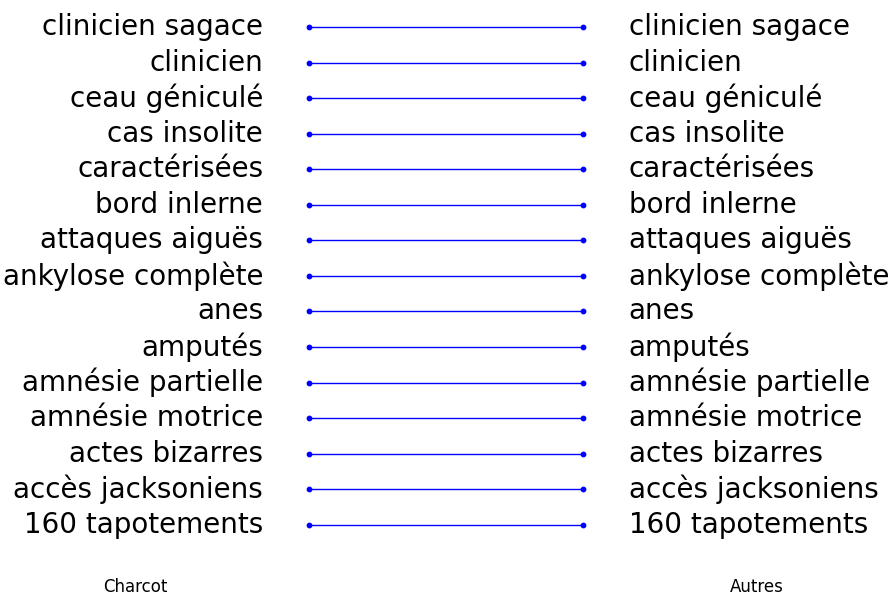
\includegraphics[width=100mm,scale=0.5]{pic/termes_partages_liens.png}
	%        \caption{Les termes communs (fréq. = 1) aux deux corpus selon \texttt{keyphrase-vectorizers}.}
	%        \label{fig:enter-label}
	%    \end{figure}
%\end{frame}

\begin{frame}{Les termes partagés les plus fréquents | \texttt{keyphrase-vectorizers}}
	\begin{figure}[!ht]
		\centering
		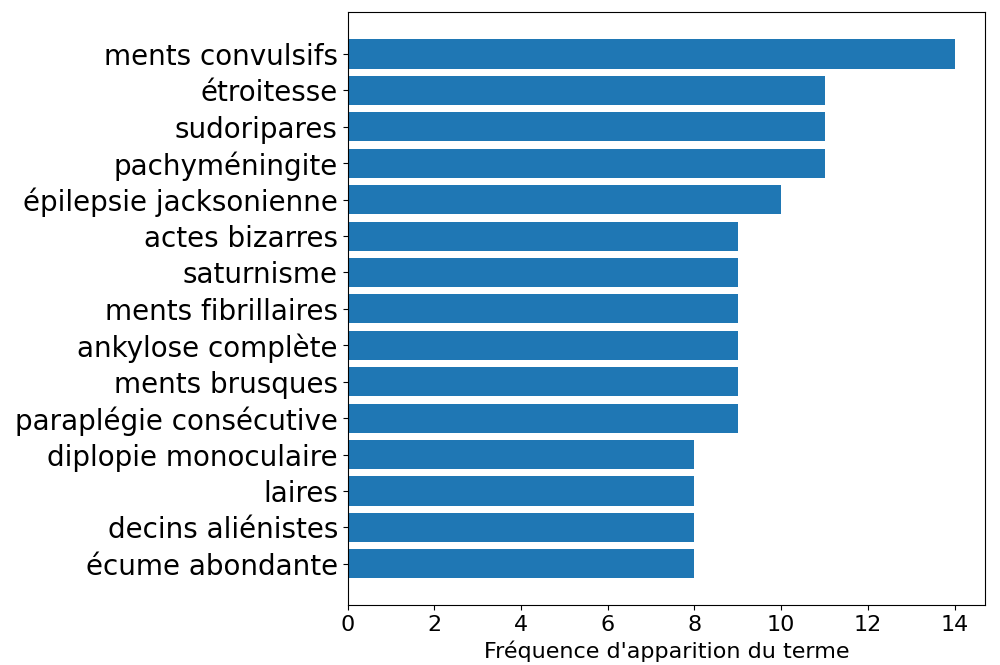
\includegraphics[width=100mm,scale=0.5]{pic/termes_partages.png}
		\caption{Les 15 termes les plus fréquents dans les deux corpus selon \texttt{keyphrase-vectorizers}.}
		\label{fig:enter-label}
	\end{figure}
\end{frame}



\begin{frame}{Analyse comparative des approches employées}
	\begin{itemize}
		\item \textit{PatternRank} valorise systématiquement les termes
		\item pas de consensus entre les métriques
		\begin{itemize}
			\item l'écart le plus petit entre eux : \textit{hypnose}
		\end{itemize}
	\end{itemize}
	\begin{figure}[h]
		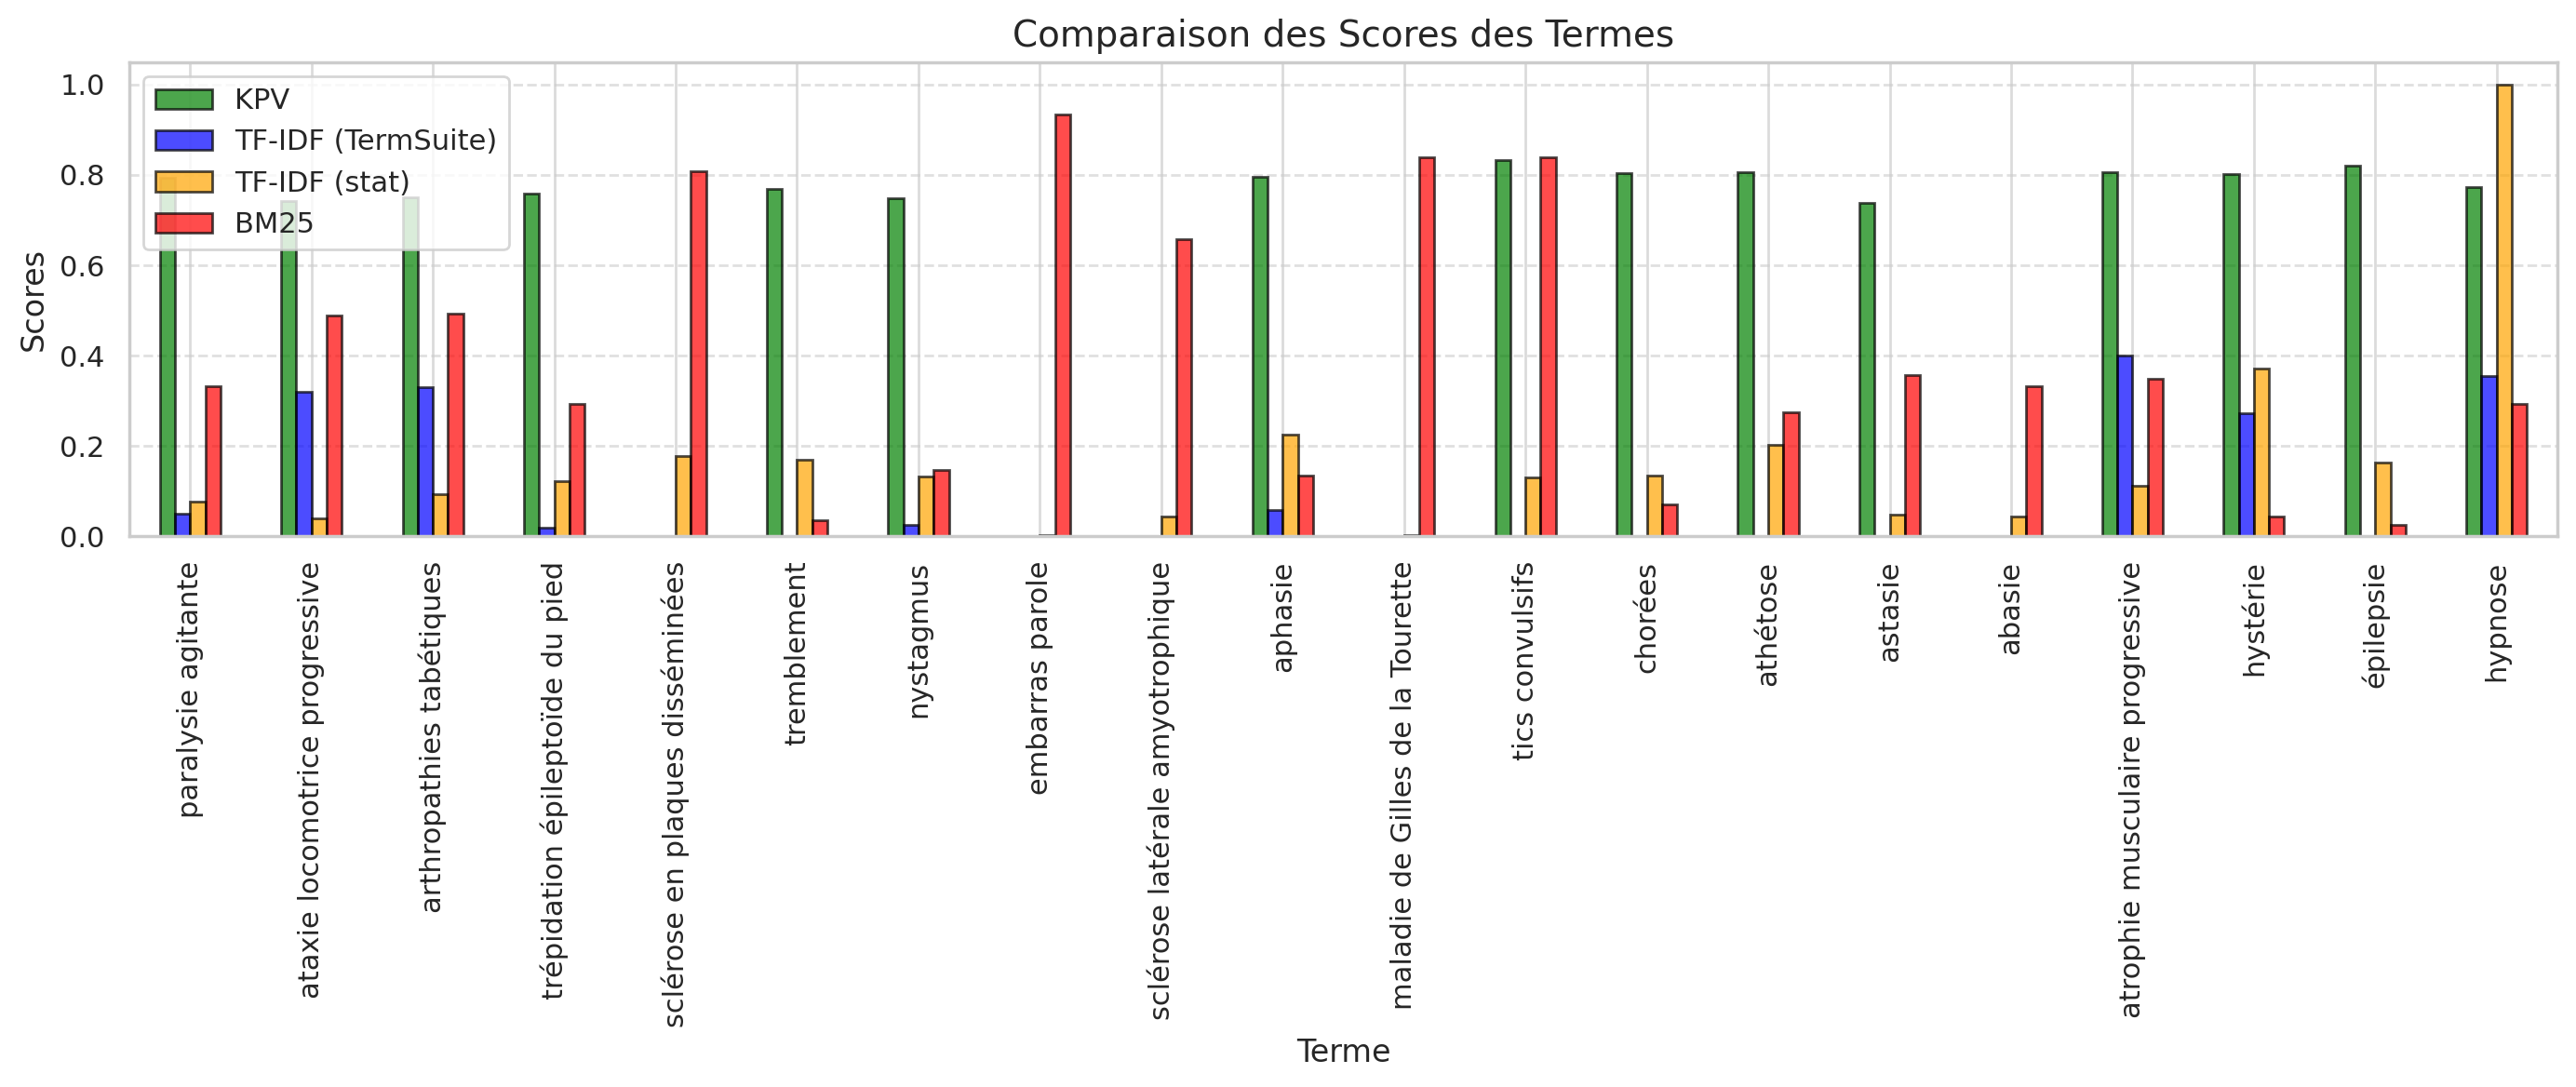
\includegraphics[width=\linewidth]{pic/termes_viz.png}
		\caption{Visualisation des scores de pertinences pour chaque terme de référence.}
		\label{fig:ling_out_TAL}
	\end{figure}
\end{frame}

%\begin{frame}{Accès à la plateforme technologique \textsc{MeSU}}
%\begin{itemize}
%\item expériences réalisées sur la plateforme \href{https://sacado.sorbonne-universite.fr/}{\textsc{MeSU}} de Sorbonne Université
%\end{itemize}
%\bigskip
%
%Les données et les scripts utilisés dans le cadre de cette étude sont disponibles sur le \href{https://github.com/ljpetkovic/JE\_IA\_HN\_030524}{dépôt GitHub}.
%\end{frame}

%\begin{frame}{Analyse comparative des approches employées}
%	\begin{itemize}
%		\item \textit{PatternRank} valorise systématiquement les termes
%		\item pas de consensus entre les métriques
%		\begin{itemize}
%			\item l'écart le plus petit entre eux : \textit{hypnose}
%		\end{itemize}
%	\end{itemize}
%	\begin{figure}[h]
%		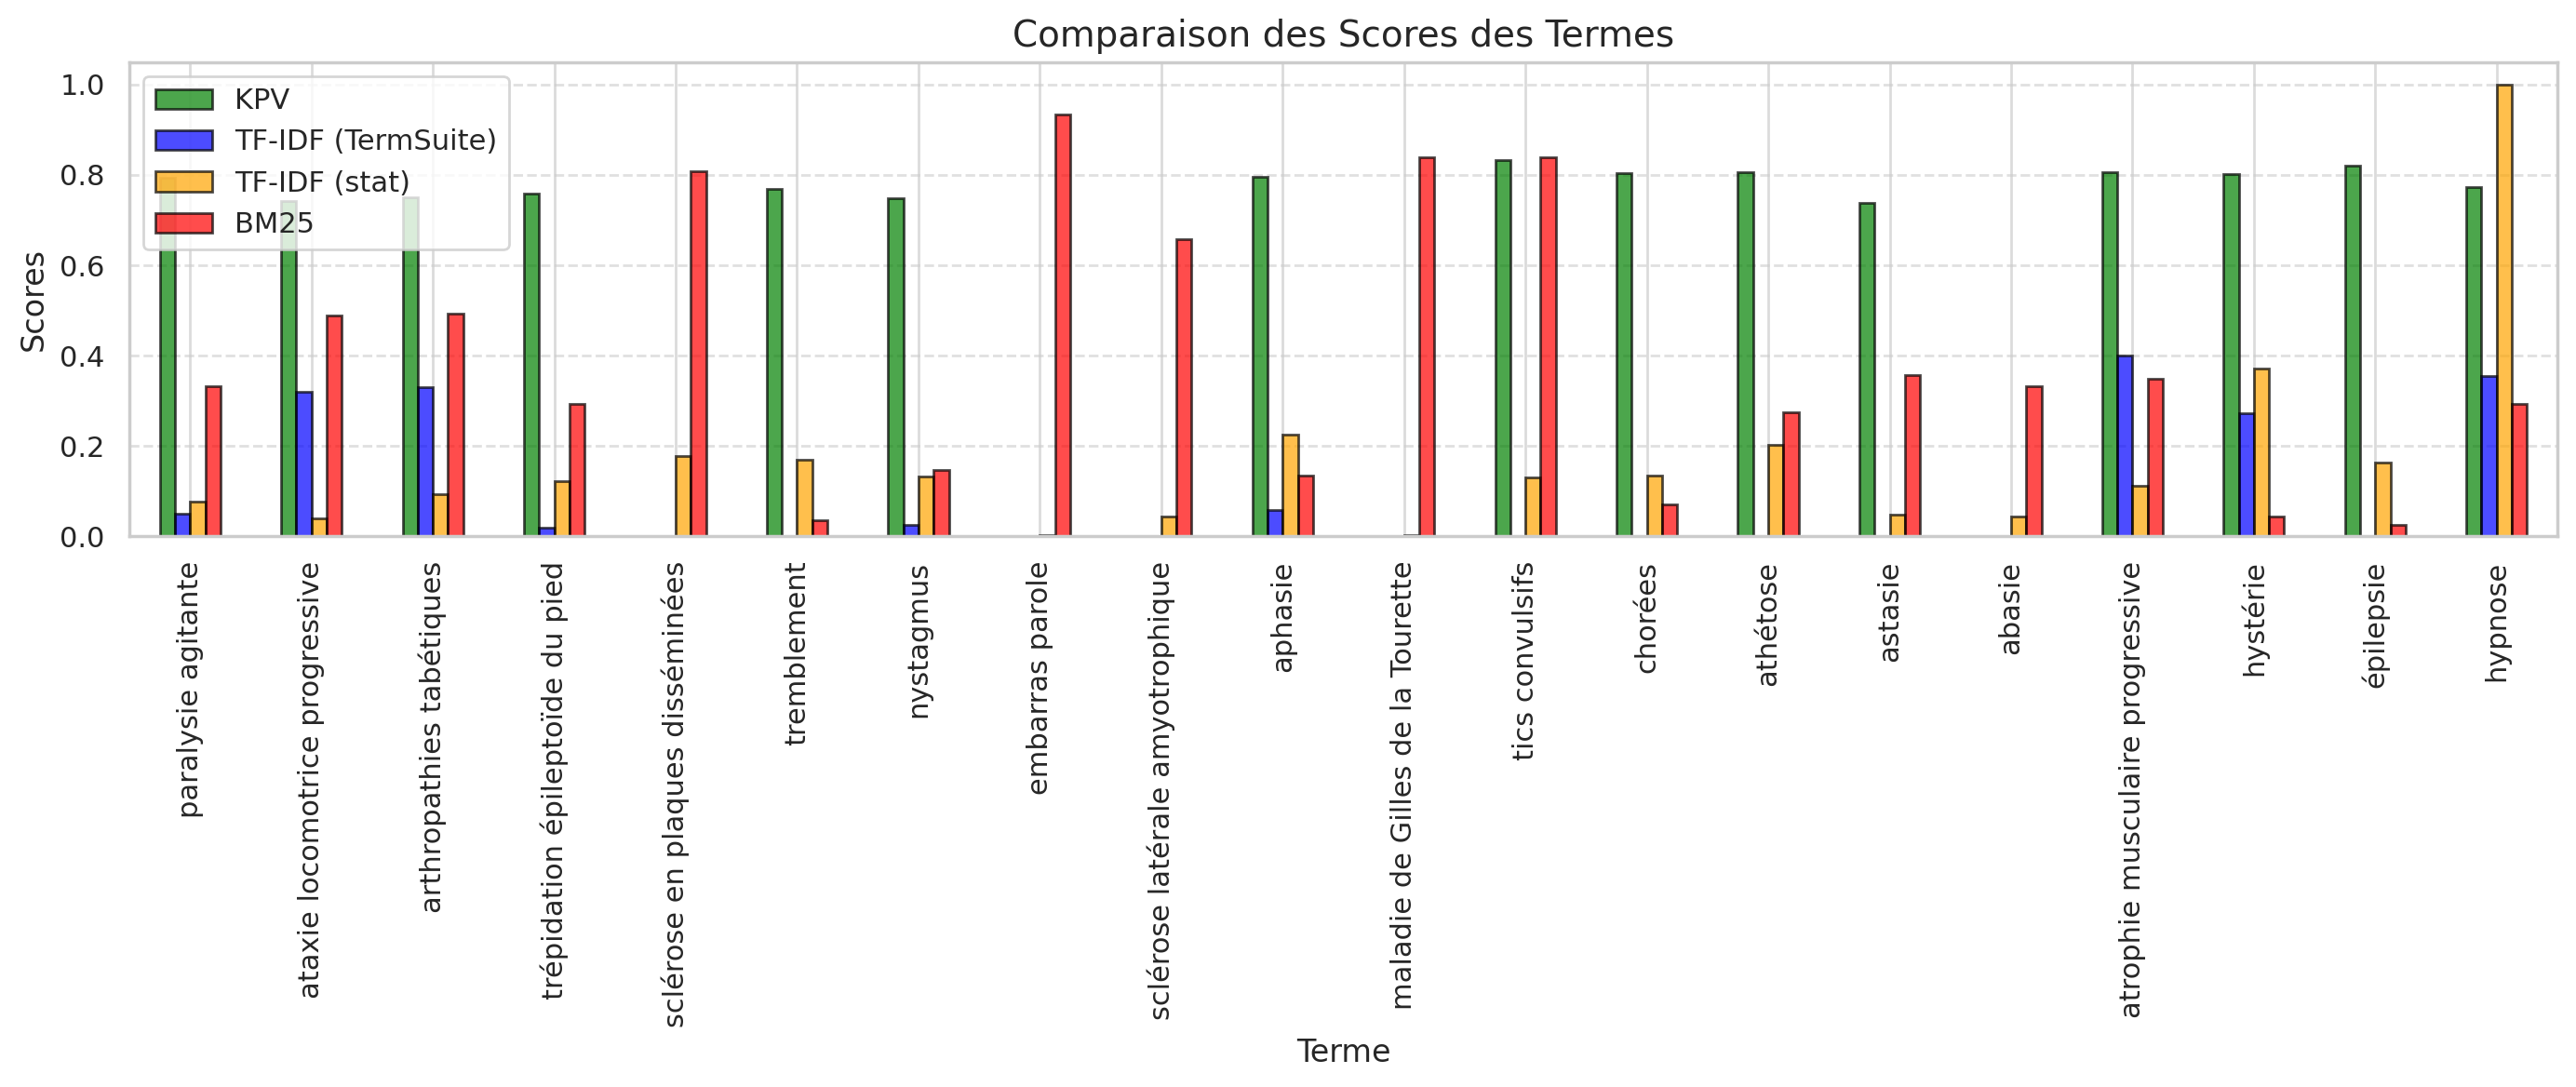
\includegraphics[width=\linewidth]{pic/termes_viz.png}
%		\caption{Visualisation des scores de pertinences pour chaque terme de référence.}
%		\label{fig:ling_out_TAL}
%	\end{figure}
%\end{frame}